\documentclass[tikz]{standalone}
\usetikzlibrary{arrows, positioning}
\tikzset{
  treenode/.style = {align=center, inner sep=1pt, text centered,
    font=\sffamily},
  bst/.style = {treenode, circle, black, font=\sffamily\bfseries, draw=black, text width=2em}, 
  sst/.style = {treenode, circle, black, font=\sffamily\bfseries, draw=red, text width=2em}, 
  txt/.style = {text width=1.5em, red},
  redline/.style={edge from parent/.style={red,very thick,-latex, draw}},
  rugularline/.style={edge from parent/.style={black, line width=0.2mm, draw}},
}
\begin{document}
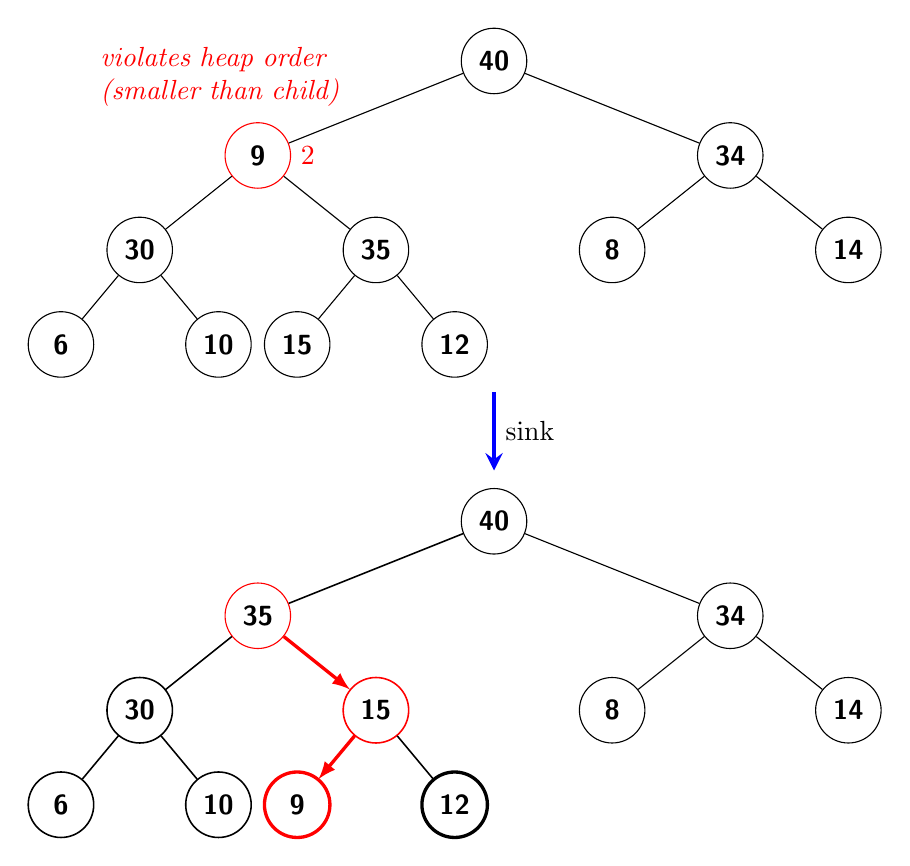
\begin{tikzpicture}[level/.style={sibling distance = 6cm/#1,
  level distance = 1.2cm}]
\node [bst] (n1) {40}
    child {node (n2) [sst] {9}
        child {node [bst] {30}
            child {node [bst] {6}}
            child {node [bst] {10}}
        }
        child {node (n5) [bst] {35}
            child {node [bst] {15}}
            child {node [bst] {12}}
        }
    }
    child { node [bst] {34}
        child{node [bst] {8}}
        child{node [bst] {14}}
    }
;
\node [right, txt] at (n2.east) {2};
\node [above, txt, text width=4cm, yshift=0.5cm] at (n2) {\textit{violates heap order \\(smaller than child)}};

\draw [stealth-, line width=0.6mm, draw=blue](0,-5.2) -- (0,-4.2)node[midway,right,shape=rectangle,draw=none]{sink};

\node [bst, below=of n1, yshift=-4cm] (2n1) {40}
    child [rugularline] {node [sst] {35}
        child [rugularline] {node [bst] {30}
            child [rugularline] {node [bst] {6}}
            child [rugularline] {node [bst] {10}}
        }
        child [redline] {node (2n5) [sst] {15}
            child [redline] {node [sst] {9}}
            child [rugularline] {node [bst] {12}}
        }
    }
    child { node [bst] {34}
        child{node [bst] {8}}
        child{node [bst] {14}}
    }
;

\end{tikzpicture}
\end{document}